\ifdefined\isMainDocument
\else
    \documentclass{article}
    \usepackage{fullpage}
    \usepackage{lineno}
    \usepackage{amsmath, amsthm, amsfonts, amssymb, amscd}
    \usepackage{bm}
    \usepackage{caption}
    \usepackage{float}
    \usepackage{graphicx}
    \graphicspath{{../main/}{../supp/}}
    \usepackage{setspace}
    \usepackage{hyperref}
    \setstretch{1.5}
    \begin{document}
    \linenumbers
    \setcounter{figure}{0}
    \renewcommand{\thefigure}{S\arabic{figure}}
\fi
% Supplementary figures (added 2026-10-20 with the Results draft), numbered S1, S2, ... by
% \beginsupplement in _main.tex, in order of first citation in Results.

\section*{Supplementary Figures}

\begin{figure}[h!]
    \centering
    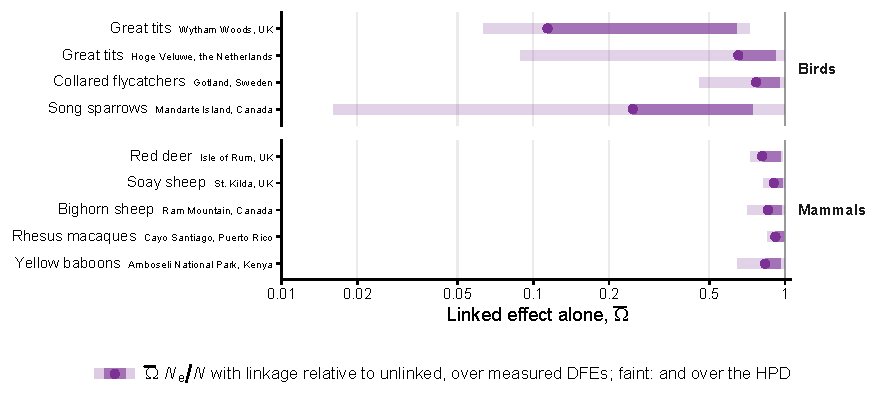
\includegraphics[width=\textwidth]{FigS_omega}
    \caption{\textbf{The linked factor is steeply nonlinear in the measured variance.} The linked factor alone, $\overline{\Omega}$, is genome-wide $N_e/N$ with linkage relative to the unlinked value at the same retention, for the nine populations with linkage maps, at the empirical DFE assigned to each population. Dot: at the posterior mode of $\hat{V}_A$; bar: over its 95\% HPD.}
    \label{fig:S_omega}
\end{figure}

\begin{figure}[h!]
    \centering
    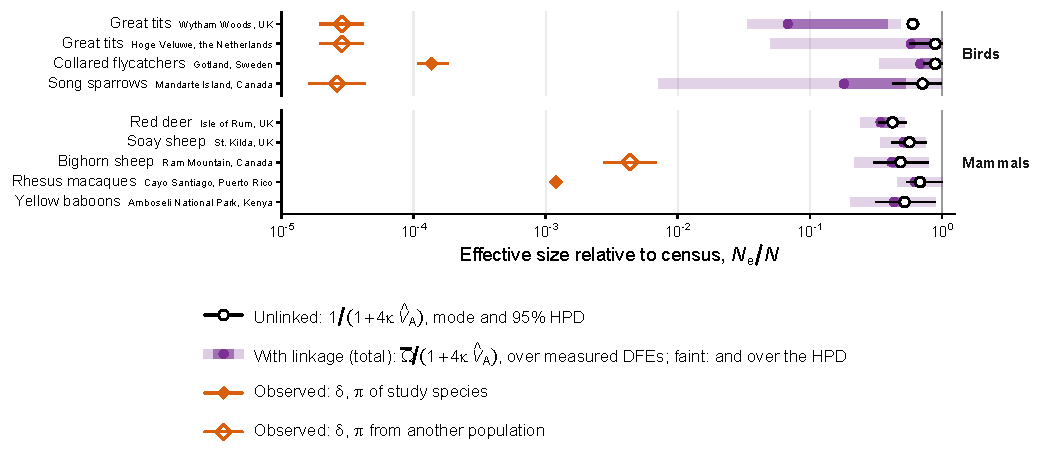
\includegraphics[width=\textwidth]{FigS_linked_fgene}
    \caption{\textbf{Partitioning the variance by gene count leaves the linked results unchanged.} As Figure~\ref{fig:linked}a, with the additive variance partitioned among chromosomes by annotated protein-coding gene count rather than by coding length.}
    \label{fig:S_fgene}
\end{figure}

\begin{figure}[h!]
    \centering
    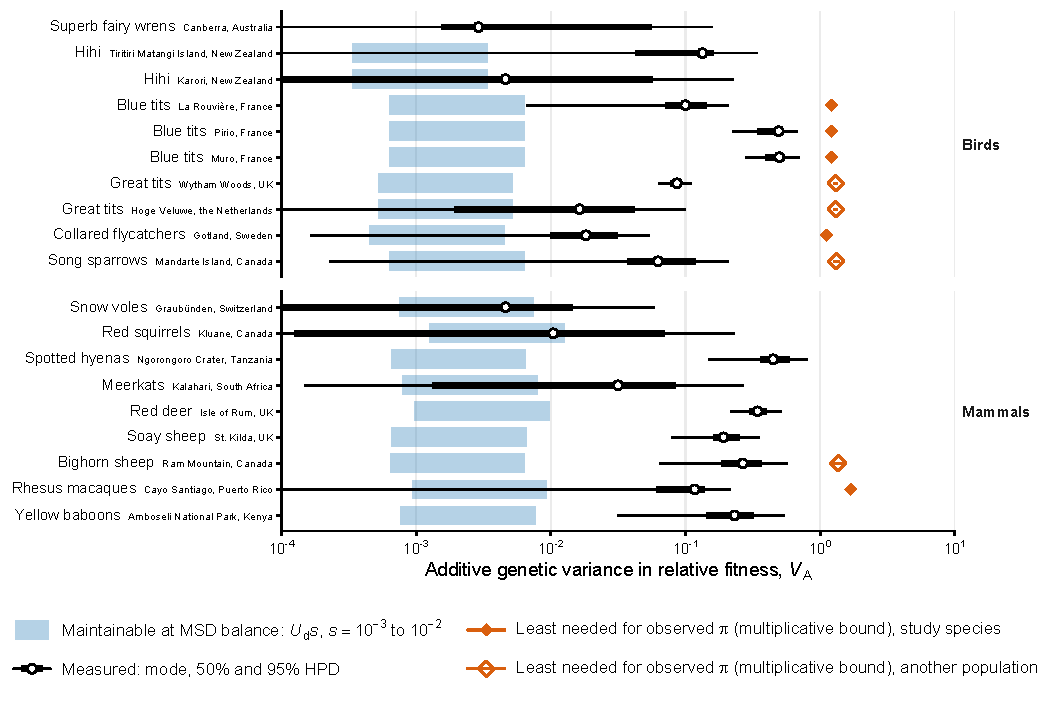
\includegraphics[width=\textwidth]{FigS_gap}
    \caption{\textbf{The measured variances lie mostly above what MSDB maintains and below what the observed deficits require.} One row per population, on a shared $V_A$ axis. Blue diamonds: the variance MSDB maintains in the strong-selection limit, $U_d\bar{s}$, with $U_d$ from the direct mutation rate and $\bar{s}$ the mean of the empirical DFE assigned to the population; where the assignment is an equal mixture of two species, the band spans $U_d$ times their means. Circles and bars: measured $\hat{V}_A$, posterior mode, 50\% (thick) and 95\% (thin) HPD. Orange diamonds: the least variance that could account for the observed deficit at unlinked sites, $V_{A,\delta}$, from $\pi$ of the study species (filled) or of another population of the species (open), with bars over the 95\% CI of the mutation rate. The superb fairy-wren has no annotated assembly; Soay sheep have no diversity estimate.}
    \label{fig:S_gap}
\end{figure}

\begin{figure}[h!]
    \centering
    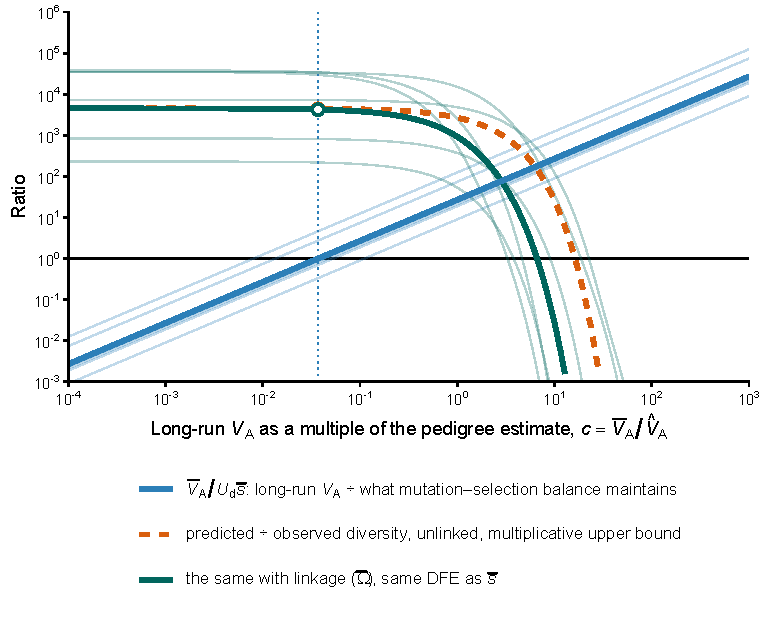
\includegraphics[width=0.85\textwidth]{FigS_rescaling_linked}
    \caption{\textbf{Linkage narrows the gap between the two tests but does not resolve it.} As Figure~\ref{fig:rescaling}, with linkage, for the six populations with both an observed deficit and a linkage map (collared flycatchers, rhesus macaques, song sparrows, bighorn sheep and both great tit populations). Blue: $\bar{V}_A/(U_d\bar{s})$. Orange dashed: predicted relative to observed diversity, unlinked, under the multiplicative bound. Green: the same with linkage, multiplied by $\overline{\Omega}(\bar{V}_A)$ at the same assigned DFE, so that both tests share a single distribution of effects. Open circle: the average at $c = U_d\bar{s}/\hat{V}_A$, where the variance is what that DFE maintains, which is the self-consistent prediction of MSDB with background selection. Bold: species averages of the $\log_{10}$ ratio (great tits averaged first); faint: populations.}
    \label{fig:S_rescaling_linked}
\end{figure}

\ifdefined\isMainDocument
\else
    \end{document}
\fi
